% $Id: omega-paper-1.tex 3930 2012-09-09 18:48:11Z jr_reuter $
%%%%%%%%%%%%%%%%%%%%%%%%%%%%%%%%%%%%%%%%%%%%%%%%%%%%%%%%%%%%%%%%%%%%%%%%
\NeedsTeXFormat{LaTeX2e}
\documentclass[12pt,a4paper]{article}
\usepackage{type1cm}
\usepackage{graphicx}
\DeclareGraphicsRule{*}{mps}{*}{}
\usepackage
  [bookmarks,bookmarksopen=true,bookmarksopenlevel=1,bookmarksnumbered=true]
  {hyperref}
\usepackage{verbatim,array,amsmath,amssymb,url}
\usepackage{thophys}
\setlength{\unitlength}{1mm}
%%%%%%%%%%%%%%%%%%%%%%%%%%%%%%%%%%%%%%%%%%%%%%%%%%%%%%%%%%%%%%%%%%%%%%%%
\widowpenalty=4000
\clubpenalty=4000
\displaywidowpenalty=4000
\allowdisplaybreaks
\renewcommand{\topfraction}{0.8}
\renewcommand{\bottomfraction}{0.8}
\renewcommand{\textfraction}{0.2}
\setlength{\abovecaptionskip}{.5\baselineskip}
\setlength{\belowcaptionskip}{\baselineskip}
%%%%%%%%%%%%%%%%%%%%%%%%%%%%%%%%%%%%%%%%%%%%%%%%%%%%%%%%%%%%%%%%%%%%%%%%
\newenvironment{algorithm}[1]%
 {\begin{list}{}%
   {\setlength{\leftmargin}{3em}%
    \setlength{\rightmargin}{3em}%
    \setlength{\itemindent}{1em}%
    \setlength{\listparindent}{0pt}%
    \settowidth{\labelwidth}{5em}%
    \renewcommand{\makelabel}[1]{\textbf{\hss##1:}}}}%
 {\end{list}}
\newenvironment{files}%
 {\begin{list}{}%
   {\setlength{\leftmargin}{3em}%
    \setlength{\rightmargin}{3em}%
    \setlength{\itemindent}{1em}%
    \setlength{\listparindent}{0pt}%
    \settowidth{\labelwidth}{5em}%
    \renewcommand{\makelabel}[1]{\texttt{##1}}}}%
 {\end{list}}
\newenvironment{options}%
 {\begin{list}{}%
   {\setlength{\leftmargin}{3em}%
    \setlength{\rightmargin}{3em}%
    \setlength{\itemindent}{1em}%
    \setlength{\listparindent}{0pt}%
    \settowidth{\labelwidth}{5em}%
    \renewcommand{\makelabel}[1]{\texttt{##1}}}}%
 {\end{list}}
%%%%%%%%%%%%%%%%%%%%%%%%%%%%%%%%%%%%%%%%%%%%%%%%%%%%%%%%%%%%%%%%%%%%%%%%
\newenvironment{code}{\verbatim}{\endverbatim\noindent}
\DeclareMathOperator{\tr}{tr}
\newcommand{\dd}{\mathrm{d}}
\newcommand{\ii}{\mathrm{i}}
\newcommand{\ee}{\mathrm{e}}
\renewcommand{\Re}{\text{Re}}
\renewcommand{\Im}{\text{Im}}
\newcommand{\ketbra}[2]{\ket{#1}\!\bra{#2}}
\newcommand{\Ketbra}[2]{\Ket{#1}\!\Bra{#2}}
\def\OCaml/{\texttt{OCaml}}
%%%%%%%%%%%%%%%%%%%%%%%%%%%%%%%%%%%%%%%%%%%%%%%%%%%%%%%%%%%%%%%%%%%%%%%%
\begin{document}
%%%%%%%%%%%%%%%%%%%%%%%%%%%%%%%%%%%%%%%%%%%%%%%%%%%%%%%%%%%%%%%%%%%%%%%%
\title{
  O'Mega: An~Optimizing~Matrix~Element~Generator.\\
  I: Basic Algorithms}
\author{%
  Mauro Moretti\thanks{\texttt{moretti@fe.infn.it}}\\
  \hfil\\
    Dipartimento di Fisica, Universit\`a di Ferrara\\
    and INFN, Sezione di Ferrara, Ferrara, Italy\\
  \hfil\\
  Thorsten Ohl\thanks{\texttt{ohl@physik.uni-wuerzburg.de},
    \texttt{http://physik.uni-wuerzburg.de/ohl}}\\
  \hfil\\
    Institut f\"ur Theoretische~Physik und Astrophysik\\
    Universit\"at~W\"urzburg\\
    Emil-Hilb-Weg 22, 97074~W\"urzburg, Germany\\
  \hfil\\
  J\"urgen Reuter\thanks{\texttt{juergen.reuter@desy.de}}\\
  \hfil\\
   Deutsches Elektronen-Synchrotron DESY\\
   Notkestra\ss{}e 85, 22607 Hamburg, Germany}
\date{%
  \fbox{\qquad LC-TOOL-2001-040 \qquad DESY 11-130 \qquad\qquad\texttt{hep-ph/0102195}\qquad}\\
  \hfil\\
  \today}
\maketitle
\newpage
\begin{abstract}
  We sketch the architecture of \textit{O'Mega}, an
  optimizing compiler for tree amplitudes in quantum field theory,
  and briefly describe its usage.
  O'Mega generates optimally efficient code for
  scattering amplitudes for many polarized particles in the Standard
  Model and its extensions.
\end{abstract}

%%%%%%%%%%%%%%%%%%%%%%%%%%%%%%%%%%%%%%%%%%%%%%%%%%%%%%%%%%%%%%%%%%%%%%%%
\section{Introduction}
\label{sec:intro}
Current and planned experiments in high energy physics can probe
physics in
processes with polarized beams and many tagged particles in the final
state.  The combinatorial explosion of the number of Feynman diagrams
contributing to scattering amplitudes for many external particles
calls for the development of more compact representations that
translate well to efficient and reliable numerical code.  In gauge
theories, the contributions from individual Feynman diagrams are gauge
dependent.  Strong numerical cancellations in a redundant
representation built from individual Feynman diagrams lead to a loss
of numerical precision, stressing further the need for eliminating
redundancies.

Due to the large number of processes that have to be studied in order
to unleash the potential of modern experiments, the construction of
nearly optimal representations must be possible algorithmically on a
computer and should not require human ingenuity for each new
application.

\textit{O'Mega}~\cite{O'Mega:Ohl} is a compiler for
tree-level scattering amplitudes that satisfies these requirements.
O'Mega is independent of the target language and can therefore create
code in any programming language for which a simple output module has
been written.  To support a physics model, O'Mega requires as input
only the Feynman rules and the relations among coupling constants.

Similar to the numerical approaches~\cite{ALPHA:1997}
and~\cite{HELAC:2000}, O'Mega reduces the growth in calculational
effort from a factorial of the number of external particles to an exponential.
The symbolic nature of O'Mega, however, increases its flexibility.
Indeed, O'Mega can emulate both~\cite{ALPHA:1997}
and~\cite{HELAC:2000} and produces code that is empirically at least
twice as fast.  The detailed description of all algorithms is
contained in the extensively commented source code of
O'Mega.

In this note, we sketch the architecture of O'Mega and describe the
usage of the first version.  The building blocks of the representation
of scattering amplitudes generated by O'Mega are described in
section~\ref{sec:1POW} and directed acyclical graphs are introduced in
section~\ref{sec:DAG}.  The algorithm for constructing the directed
acyclical graph is presented in section~\ref{sec:algorithm} and its
implementation is described in section~\ref{sec:implementation}.
We conclude with a few results and examples in
section~\ref{sec:results}.  Practical information is
presented in the appendices: installation of the O'Mega software in
appendix~\ref{sec:installation}, running of the O'Mega compiler in
appendix~\ref{sec:running} and using O'Mega's output in
appendix~\ref{sec:using}.  Finally, appendix~\ref{sec:extensions}
briefly discusses mechanisms for extending O'Mega.


%%%%%%%%%%%%%%%%%%%%%%%%%%%%%%%%%%%%%%%%%%%%%%%%%%%%%%%%%%%%%%%%%%%%%%%%
\section{One-Particle Off-Shell Wave Functions}
\label{sec:1POW}

\textit{One-Particle Off-Shell Wave Functions}~(1POWs) are obtained
from connected Green's functions by applying the LSZ reduction formula
to all but one external line while the remaining line is kept off the
mass shell
\begin{multline}
  W(x; p_1,\ldots,p_n; q_1,\ldots,q_m) = \\
    \Braket{\phi(q_1),\ldots,\phi(q_m);\text{out}|\Phi(x)
           |\phi(p_1),\ldots,\phi(p_n);\text{in}}\,.
\end{multline}
Depending on the context, the off-shell line will either be understood as
amputated or not.  For example,
$\Braket{\phi(q_1),\phi(q_2);\text{out}|\Phi(x)|\phi(p_1);\text{in}}$
in unflavored scalar $\phi^3$-theory is given at tree level by
\begin{equation}
  \parbox{26\unitlength}{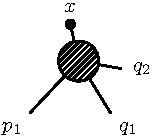
\includegraphics{omega-paper-1-pics-1}} =
  \parbox{26\unitlength}{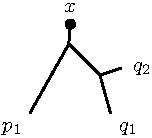
\includegraphics{omega-paper-1-pics-2}} +
  \parbox{26\unitlength}{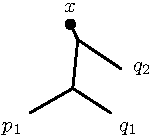
\includegraphics{omega-paper-1-pics-3}} +
  \parbox{26\unitlength}{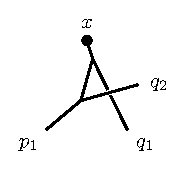
\includegraphics{omega-paper-1-pics-4}}.
\end{equation}

The number of distinct momenta that can be formed from
$n$~external momenta is $P(n)=2^{n-1}-1$.  Therefore, the number of
tree 1POWs grows exponentially with the number of external particles
and not with a factorial, as the number of Feynman diagrams, e.\,g.{}
$F(n)=(2n-5)!!=(2n-5)\cdot\ldots5\cdot3\cdot1$ in unflavored
$\phi^3$-theory.

At tree-level, the set of all 1POWs for a given set of external
momenta can be constructed recursively
\begin{equation}
\label{eq:recursive-1POW}
  \parbox{22\unitlength}{
\includegraphics{omega-paper-1-pics-5}} = 
  \sum_{k+l=n}
  \parbox{32\unitlength}{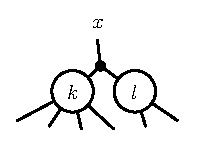
\includegraphics{omega-paper-1-pics-6}}\,,
\end{equation}
where the sum extends over all partitions of the set of $n$~momenta.
This recursion will terminate at the external wave functions.

For all quantum field theories, there are---well defined, but not
unique---sets of \emph{Keystones}~$K$ such that the sum
of tree Feynman diagrams for a given process can be expressed as a
sparse sum of products of 1POWs without double counting.  In a theory
with only cubic couplings this is expressed as
\begin{equation}
\label{eq:keystones}
  T = \sum_{i=1}^{F(n)} D_i =
      \sum_{k,l,m=1}^{P(n)}
        K^{3}_{f_kf_lf_m}(p_k,p_l,p_m)
        W_{f_k}(p_k)W_{f_l}(p_l)W_{f_m}(p_m)\,,
\end{equation}
with obvious generalizations.
The non-trivial problem is to avoide the
double counting of diagrams like
\begin{center}
   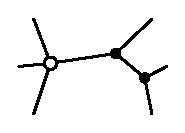
\includegraphics{omega-paper-1-pics-7}
   \qquad\qquad
   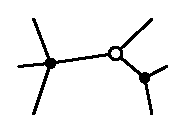
\includegraphics{omega-paper-1-pics-8}\,,
\end{center} 
where the circle denotes the keystone. The problem has been solved
explicitly for general theories with vertices of arbitrary
degrees.  The solution is inspired by
arguments~\cite{ALPHA:1997} based on the equations of motion (EOM) of
the theory in the presence of sources. The iterative solution of the
EOM leads to the construction of the 1POWs and the constraints imposed
on the 1POWs by the EOM suggest the correct set~\cite{ALPHA:1997} of
partitions $\{(p_k,p_l,p_m)\}$ in equation~(\ref{eq:keystones}).

The maximally symmetric solution selects among equivalent diagrams the
keystone closest to the center of a diagram.  This corresponds to
the numerical expressions of~\cite{ALPHA:1997}.  The absence of double
counting can be demonstrated by counting the number~$F(d_{\max},n)$ of
unflavored Feynman tree diagrams with~$n$ external legs and vertices of
maximum degree~$d_{\max}$ in two different ways: once directly and then
as a sum over keystones.  The number~$\tilde F(d_{\max},N_{d,n})$ of
unflavored Feynman tree diagrams for one keystone
$N_{d,n}=\{n_1,n_2,\ldots,n_d\}$, with $n = n_1 + n_2 + \cdots + n_d$,
is given by the product of the number of subtrees and symmetry factors
\begin{subequations}
\begin{equation}
  \tilde F(d_{\max},N_{d,n}) =
    \frac{n!}{|\mathcal{S}(N_{d,n})|\sigma(n_d,n)}
    \prod_{i=1}^{d} \frac{F(d_{\max},n_i+1)}{n_i!}\,
\end{equation}
where $|\mathcal{S}(N)|$ is the size of the symmetric group
of~$N$, $\sigma(n,2n) = 2$ and $\sigma(n,m) = 1$ otherwise.  Indeed,
it can be verified that the sum over all keystones reproduces the
number
\begin{equation}
  F(d_{\max},n) =
    \sum_{d=3}^{d_{\max}}
    \sum_{\substack{N = \{n_1,n_2,\ldots,n_d\}\\
                    n_1 + n_2 + \cdots + n_d = n\\
                    1 \le n_1 \le n_2 \le \cdots \le n_d \le \lfloor n/2 \rfloor}}
     \tilde F(d_{\max},N)
\end{equation}
\end{subequations}
of \emph{all} unflavored Feynman tree diagrams.

A second consistent prescription for the construction of keystones is
maximally asymmetric and selects the keystone adjacent to a chosen
external line.  This prescription reproduces the approach
in~\cite{HELAC:2000} where the tree-level Schwinger-Dyson equations
are used as a special case of the EOM.

Interfering color amplitudes are implemented by using O'Mega's basic
algorithm for the Feynman rules in the color flow
basis~\cite{OMEGA2,cflow}.  In the case of Dirac fermions, Fermi
statistics can be implemented straightforwardly in the 1POWs by
maintaining a list of the ordered pairs of external fermions connected
by directed fermion lines.  This approach can be
generalized~\cite{OMEGA2} for models with Majorana fermions and
fermion number violating interactions, such as supersymmetric models
using the Feynman rules of~\cite{Denner/etal:Majorana}.

Recursive algorithms for gauge theory amplitudes have been pioneered
in~\cite{Berends:1988me}.  The use of 1POWs as basic building blocks
for the calculation of scattering amplitudes in tree approximation has
been advocated in~\cite{HELAS} and a heuristic procedure, without
reference to keystones, for minimizing the number of arithmetical
operations has been suggested.  This approach is used by
MADGRAPH~\cite{MADGRAPH} for fully automated calculations. The
heuristic optimizations are quite efficient for $2\to4$ processes, but
the number of operations remains bounded from below by the number of
Feynman diagrams.  In the time since O'Mega was first made available
publically, more programs using a recursive construction of amplitudes
have been published, e.\,g.~Comix~\cite{Comix}.

%%%%%%%%%%%%%%%%%%%%%%%%%%%%%%%%%%%%%%%%%%%%%%%%%%%%%%%%%%%%%%%%%%%%%%%%
\subsection{Ward Identities}
\label{sec:WI}

\begin{subequations}
A particularly convenient property of the 1POWs in gauge theories is
that, even for vector particles, the 1POWs are `almost' physical
objects and satisfy simple Ward Identities
\label{eq:ward}
\begin{equation}
    \frac{\partial}{\partial x_\mu}
    \Braket{\text{out}|A_\mu(x)|\text{in}}_{\text{amp.}} = 0
\end{equation}
for unbroken gauge theories and
\begin{equation}
    \frac{\partial}{\partial x_\mu}
    \Braket{\text{out}|W_\mu(x)|\text{in}}_{\text{amp.}} =
      - m_W \Braket{\text{out}|\phi_W(x)|\text{in}}_{\text{amp.}}
\end{equation}
for spontaneously broken gauge theories in $R_\xi$-gauge for all
physical external states~$\ket{in}$ and $\ket{out}$. Thus the
identities~(\ref{eq:ward}) can serve as powerful numerical checks
both for the consistency of a set of Feynman rules and for the
numerical stability of the generated code.   The code for matrix
elements can optionally be instrumented by O'Mega with numerical
checks of these Ward identities for intermediate lines.
\end{subequations}

%%%%%%%%%%%%%%%%%%%%%%%%%%%%%%%%%%%%%%%%%%%%%%%%%%%%%%%%%%%%%%%%%%%%%%%%
\section{Directed Acyclical Graphs}
\label{sec:DAG}

The algebraic expression for the tree-level scattering amplitude in
terms of Feynman diagrams is itself a tree.  The much slower growth of
the set of 1POWs compared to the set of Feynman diagrams shows that this
representation is extremely redundant. In this case, \emph{Directed
Acyclical Graphs} (DAGs) provide a more efficient representation, as
illustrated by a trivial example
\begin{equation}
  ab (ab+c) =
  \parbox{28\unitlength}{\hfil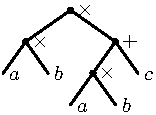
\includegraphics{omega-paper-1-pics-9}\hfil}
    = \parbox{18\unitlength}{\hfil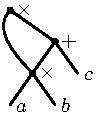
\includegraphics{omega-paper-1-pics-10}\hfil}
\end{equation}
where one multiplication is saved.  The replacement of expression
trees by equivalent DAGs is part of the repertoire of optimizing
compilers, known as \emph{common subexpression elimination}.
Unfortunately, this approach fails in practice for all interesting
expressions appearing in quantum field theory, because of the
combinatorial growth of space and time required to find an almost
optimal factorization.

However, the recursive definition in equation~(\ref{eq:recursive-1POW})
allows to construct the DAG of the 1POWs in equation~(\ref{eq:keystones})
\emph{directly} ~\cite{O'Mega:Ohl}, without having to construct and
factorize the Feynman diagrams explicitly.

As mentioned above, there is more than one consistent prescription for
constructing the set of keystones.  The symbolic
expressions constructed by O'Mega contain the symbolic equivalents of
the numerical expressions computed by~\cite{ALPHA:1997} (maximally
symmetric keystones) and~\cite{HELAC:2000} (maximally asymmetric
keystones) as special cases.

%%%%%%%%%%%%%%%%%%%%%%%%%%%%%%%%%%%%%%%%%%%%%%%%%%%%%%%%%%%%%%%%%%%%%%%%
\section{Algorithm}
\label{sec:algorithm}

By virtue of their recursive construction
in~(\ref{eq:recursive-1POW}), tree-level 1POWs form a DAG and the
problem is to find the \emph{smallest} DAG that corresponds to a given tree,
(i.\,e.~a given sum of Feynman diagrams).  O'Mega's algorithm
proceeds in four steps
\begin{algorithm}{Calculate}
  \item[Grow] starting from the external particles, build the tower of
    \emph{all} 1POWs up to a given height (the height
    is less than the number of external lines for asymmetric
    keystones and less than half of that for symmetric keystones)
    and translate it to the equivalent DAG~$D$.
  \item[Select] from $D$, determine \emph{all} possible
    \emph{flavored keystones} for the process under
    consideration and the 1POWs appearing in them.
  \item[Harvest] construct a sub-DAG $D^*\subseteq D$ consisting
    \emph{only} of nodes that contribute to the 1POWs
    appearing in the flavored keystones.
  \item[Calculate] multiply the 1POWs as specified by the keystones
    and sum the keystones.
\end{algorithm}
By construction, the resulting expression contains no more
redundancies and can be translated to a numerical expression.  In
general, asymmetric keystones create an expression that is smaller
by a few percent than the result from symmetric keystones, but it
is not obvious which approach produces the numerically more robust
results.

The details of this algorithm as implemented in O'Mega are described
in the source code.  The persistent data
structures~\cite{Okasaki:1998:book} used for the determination
of~$D^*$ are very efficient. The generation of Fortran
code for amplitudes in the Standard Model is always much faster than
the subsequent compilation.

%%%%%%%%%%%%%%%%%%%%%%%%%%%%%%%%%%%%%%%%%%%%%%%%%%%%%%%%%%%%%%%%%%%%%%%%
\section{Implementation}
\label{sec:implementation}
The O'Mega compiler is implemented in \OCaml/~\cite{OCaml}, a
functional programming language of the ML family with a very
efficient, portable and freely available implementation, that can be
bootstrapped on all modern computers in a few minutes.

The powerful module system of \OCaml/ allows an efficient and concise
implementation of the DAGs for a specific physics model as a functor
application.  This functor maps from the category of
trees to the category of DAGs and is applied to the set of trees
defined by the Feynman rules of any model under consideration.

\begin{figure}
  %includegraphics[width=\textwidth]{modules}
  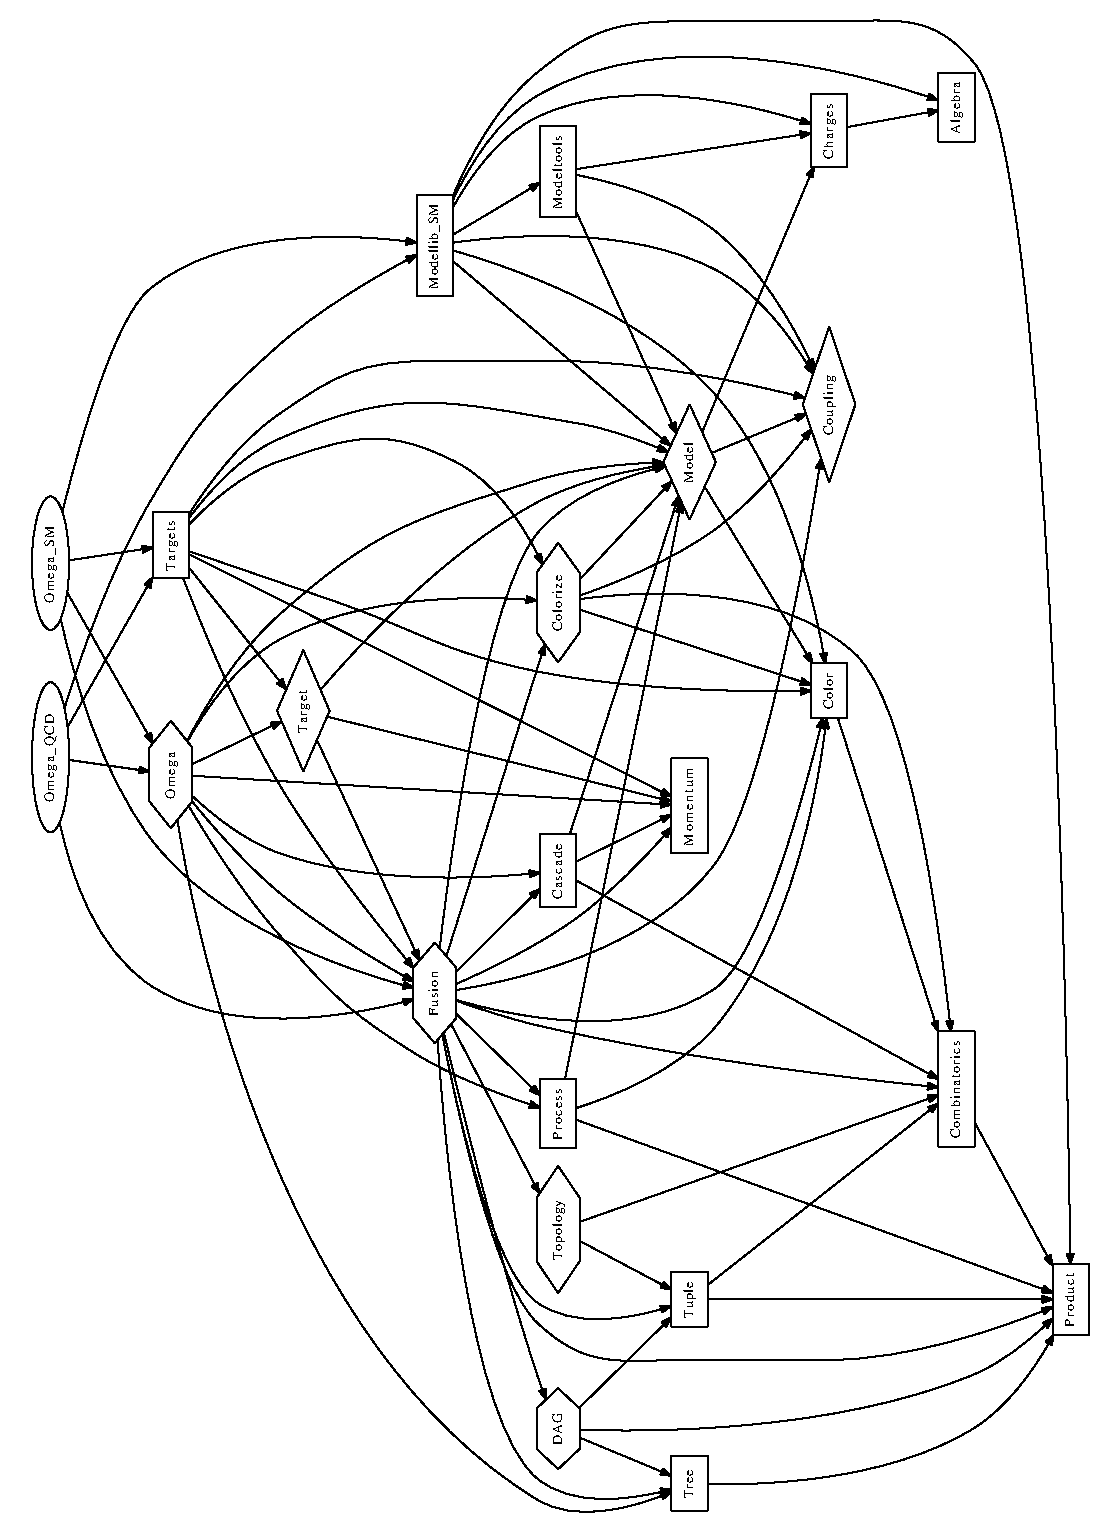
\includegraphics[height=.9\textheight]{modules}
  \caption{\label{fig:modules}%
    Major module dependencies in O'Mega.  The diamond shaped nodes denote
    abstract signatures defining functor domains and co-domains.
    The hexagons denote functors and
    rectangular boxes denote modules, while oval
    boxes stand for example applications.}
\end{figure}
The module system of \OCaml/ has been used to make the combinatorial
core of O'Mega demonstrably independent from the specifics of both the
physics model and the target language, as shown in
Figure~\ref{fig:modules}.  A Fortran backend has been realized
first.  The electroweak Standard Model and the Minimal Supersymmetric
Standard Model~(MSSM) have been implemented and tested
extensively~\cite{Hagiwara:2005wg}.  Many extensions of these models
and more exotic models are available in the distribution.

Many extensions of the Standard Model, most prominently the MSSM,
contain Majorana fermions.  In
this case, fermion lines have no canonical orientation and the
determination of the relative signs of interfering amplitudes is not
trivial.  However, the Feynman rules for Majorana fermions and fermion
number violating interactions proposed in~\cite{Denner/etal:Majorana}
have been implemented in O'Mega~\cite{OMEGA2} in analogy to the Feynman rules
for Dirac fermions and both methods are available.  Numerical
comparisons of amplitudes for Dirac fermions calculated both ways show
agreement at a small multiple of the machine precision.

As mentioned above, the compilers for the target programming language
are the slowest step in the generation of executable code.  On the
other hand, the execution speed of the code is limited by non-trivial
vertex evaluations for vectors and spinors, which need $O(10)$ complex
multiplications.  Therefore, an \emph{O'Mega Virtual Machine} can
challenge native code and avoid compilations.

%%%%%%%%%%%%%%%%%%%%%%%%%%%%%%%%%%%%%%%%%%%%%%%%%%%%%%%%%%%%%%%%%%%%%%%%
\section{Results}
\label{sec:results}

%%%%%%%%%%%%%%%%%%%%%%%%%%%%%%%%%%%%%%%%%%%%%%%%%%%%%%%%%%%%%%%%%%%%%%%%
\subsection{Examples}
\label{sec:examples}

\begin{table}
  \begin{center}
    \begin{tabular}{l|rr|rr}
                    \multicolumn{1}{c|}{process}
                  & \multicolumn{2}{c|}{Diagrams}
                  & \multicolumn{2}{c}{O'Mega} \\
                  & \multicolumn{1}{c}{\#} & vertices
                  & \#prop. & vertices \\%\hline
      $e^+e^-\to e^+\bar\nu_e d\bar u$
        &     20 &      80 &  14 &   45 \\
%%%SM4  &     20 &      80 &  14 &   45 \\
%%%SM4h &     20 &      80 &  14 &   35 \\
      $e^+e^-\to e^+\bar\nu_e d\bar u \gamma$
        &    146 &     730 &  36 &  157 \\
%%%SM4  &    142 &     710 &  33 &  151 \\
%%%SM4h &    142 &     710 &  33 &  115 \\
      $e^+e^-\to e^+\bar\nu_e d\bar u \gamma\gamma$
        &   1256 &    7536 &  80 &  462 \\
%%%SM4  &   1174 &    7044 &  71 &  441 \\
%%%SM4h &   1174 &    7044 &  71 &  361 \\
      $e^+e^-\to e^+\bar\nu_e d\bar u \gamma\gamma\gamma$
        &  12420 &   86940 & 168 & 1343 \\
%%%SM4  &  11058 &   77406 & 147 & 1284 \\
%%%SM4h &  11058 &   77406 & 147 & 1106 \\
      $e^+e^-\to e^+\bar\nu_e d\bar u \gamma\gamma\gamma\gamma$
        & 138816 & 1110528 & 344 & 3933
    \end{tabular}
  \end{center}
  \caption{\label{tab:4fgamma}%
    Radiative corrections to four fermion production: comparison of
    the computational complexity of scattering amplitudes obtained
    from Feynman diagrams and from O'Mega. (The counts correspond to
    the full Standard Model---sans light fermion Yukawa couplings---in
    unitarity gauge with quartic couplings emulated by cubic 
    couplings of non-propagating auxiliary fields.)}
\end{table}

\begin{table}
  \begin{center}
    \begin{tabular}{l|rr|rr}
                    \multicolumn{1}{c|}{process}
                  & \multicolumn{2}{c|}{Diagrams}
                  & \multicolumn{2}{c}{O'Mega} \\
                  & \multicolumn{1}{c}{\#} & vertices
                  & \#prop. & vertices \\%\hline
      $e^+e^-\to e^+\bar\nu_e d\bar u b\bar b$
        &    472 &   2832 &  49 &   232 \\
%%%SM4  &    464 &   2784 &  46 &   227 \\
%%%SM4h &    464 &   2784 &  46 &   186 \\
      $e^+e^-\to e^+\bar\nu_e d\bar u b\bar b \gamma$
        &   4956 &  34692 & 108 &   722 \\
%%%SM4  &   4738 &  33166 &  99 &   709 \\
%%%SM4h &   4738 &  33166 &  99 &   606 \\
      $e^+e^-\to e^+\bar\nu_e d\bar u b\bar b \gamma\gamma$
        &  58340 & 466720 & 226 &  2212
    \end{tabular}
  \end{center}
  \caption{\label{tab:6fgamma}%
    Radiative corrections to six fermion production: comparison of
    the computational complexity of scattering amplitudes obtained
    from Feynman diagrams and from O'Mega. (The counts correspond to
    the full Standard Model---sans light fermion Yukawa couplings---in
    unitarity gauge with quartic couplings emulated by cubic 
    couplings of non-propagating auxiliary fields.)}
\end{table}

Tables~\ref{tab:4fgamma} and~\ref{tab:6fgamma} show the reduction in
computational complexity for some important processes at a
$e^+e^-$-linear collider including radiative corrections.  Using the
asymmetric keystones can reduce the number of vertices by some~10
to~20 percent relative to the quoted numbers for symmetric keystones.

%%%%%%%%%%%%%%%%%%%%%%%%%%%%%%%%%%%%%%%%%%%%%%%%%%%%%%%%%%%%%%%%%%%%%%%%
\subsection{Comparisons}
\label{sec:comparisons}

HELAC's~\cite{HELAC:2000} diagnostics report more vertices than O'Mega
for identical amplitudes.  This ranges from comparable numbers for
Standard Model processes with many different flavors to an increase by
50 percent for processes with many identical flavors.  Empirically,
O'Mega's straight line code is twice as fast as HELAC's DO-loops for
identical optimizing Fortran compilers (not counting HELAC's
initialization phase).  Together this results in an improved
performance by a factor of two to three.

The numerical efficiency of O'Mega's Fortran runtime library is
empirically identical to HELAS~\cite{HELAS}. Therefore, O'Mega's
performance can directly be compared to
MADGRAPH's~\cite{MADGRAPH} by comparing the number of vertices.
For $2\to5$-processes in the Standard Model, O'Mega's advantage in
performance is about a factor of two and grows from there.

The results have been compared with MADGRAPH~\cite{MADGRAPH} for
many Standard Model processes and numerical agreement at the level
of~$10^{-11}$ has been found with double precision floating point
arithmetic.

%%%%%%%%%%%%%%%%%%%%%%%%%%%%%%%%%%%%%%%%%%%%%%%%%%%%%%%%%%%%%%%%%%%%%%%%
\subsection{Applications}
O'Mega generated amplitudes are used in the multi-purpose
event generator generator WHIZARD~\cite{WHIZARD}.  The first
complete experimental study of vector boson scattering in six fermion
production for linear collider
physics~\cite{Chierici/Kobel/Rosati:2000:TDR-backup} was
facilitated by O'Mega and WHIZARD.

%%%%%%%%%%%%%%%%%%%%%%%%%%%%%%%%%%%%%%%%%%%%%%%%%%%%%%%%%%%%%%%%%%%%%%%%
\section*{Acknowledgments}
We thank Wolfgang Kilian for providing the WHIZARD Monte Carlo
generator environment that turns our numbers into real events with
unit weight.  Thanks to the ECFA/DESY Linear Collider workshops and
their participants for providing a showcase.  Parts of this research
were supported by Bundesministerium f\"ur Bildung und Forschung
(Germany), Deutsche Forschungsgemeinschaft and the Helmholtz Alliance
\textit{Physics at the Terascale}.

Finally, thanks to the \OCaml/ team at INRIA for the
lean and mean implementation of a programming language that does not
insult the programmer's intelligence.

%%%%%%%%%%%%%%%%%%%%%%%%%%%%%%%%%%%%%%%%%%%%%%%%%%%%%%%%%%%%%%%%%%%%%%%%
\begin{thebibliography}{10}
  \bibitem{O'Mega:Ohl}
    T. Ohl, \textit{O'Mega: An~Optimizing Matrix~Element~Generator},
    Proceedings of the \textit{Workshop on Advanced Computing and
    Analysis Technics in Physics Research,} Fermilab, October 2000,
    IKDA 2000/30, [arXiv:hep-ph/0011243];
    T. Ohl, \textit{O'Mega \&\ WHIZARD: Monte Carlo Event Generator
    Generation For Future Colliders}, Proceedings of the
    \textit{Workshop on Physics and Experimentation with Future Linear
    $e^+e^-$-Colliders (LCWS2000),} Fermilab, October 2000,
    IKDA 2000/31, [arXiv:hep-ph/0011287].
  \bibitem{ALPHA:1997}
    F.~Caravaglios, M.~Moretti,
    Phys.{} Lett.{} \textbf{B358} (1995) 332,
    [arXiv:hep-ph/9507237];
    Z.{} Phys.{} \textbf{C74} (1997) 291,
    [arXiv:hep-ph/9604316].
%%\bibitem{Alpgen}
%%  M.~L.~Mangano, M.~Moretti, F.~Piccinini, R.~Pittau, A.~D.~Polosa,
%%  JHEP \textbf{0307} (2003) 001,
%%  [arXiv:hep-ph/0206293].
  \bibitem{HELAC:2000}
    A.~Kanaki, C.~G.~Papadopoulos,
    Comput.{} Phys.{} Commun.{} \textbf{132 } (2000) 306,
    [arXiv:hep-ph/0002082].
  \bibitem{OMEGA2}
    W. Kilian, T. Ohl, J. Reuter,
    \textit{O'Mega: An~Optimizing~Matrix~Element~Generator.
    II: Amplitudes~With~Color~Flow and Without~Fermion~Number~Conservation},
    to be published.
  \bibitem{cflow}
    W.~Kilian, T.~Ohl, J.~Reuter, C.~Speckner,
    \textit{QCD in the Color-Flow Representation},
    to be published.
  \bibitem{Denner/etal:Majorana}
    A. Denner, H. Eck, O. Hahn, J. K\"ublbeck,
    Phys.{} Lett.{}  \textbf{B291} (1992) 278;
    Nucl.{} Phys.{}  \textbf{B387} (1992) 467.
  \bibitem{Berends:1988me}
    F.~A.~Berends, W.~T.~Giele,
    Nucl.{} Phys.{} \textbf{B306} (1988) 759.
  \bibitem{HELAS}
    H. Murayama, I. Watanabe, K. Hagiwara,
    \textit{HELAS: HELicity amplitude subroutines for Feynman diagram
      evaluations},
    KEK Report 91-11.
  \bibitem{MADGRAPH}
    T. Stelzer, W. F. Long,
    Comput.{} Phys.{} Commun.{} \textbf{81} (1994) 357,
    [arXiv:hep-ph/9401258].
    %%% J.~Alwall, M.~Herquet, F.~Maltoni, O.~Mattelaer, T.~Stelzer,
    %%% JHEP \textbf{1106} (2011)  128,
    %%% [arXiv:1106.0522].
  \bibitem{Comix}
    T.~Gleisberg, S.~Hoeche,
    JHEP \textbf{0812} (2008)  039,
    [arXiv:0808.3674].
  \bibitem{Okasaki:1998:book}
    Chris Okasaki,
    \textit{Purely Functional Data Structures},
    Cambridge University Press, 1998.
  \bibitem{OCaml}
    Xavier Leroy et al.,
    \textit{The \OCaml/ System, Release 3.12, Documentation and User's Manual},
    Technical Report, INRIA, 2011,
    \url{http://pauillac.inria.fr/ocaml/}.
  \bibitem{Hagiwara:2005wg}
    K.~Hagiwara \textit{et al.},
    Phys.{} Rev.{} \textbf{D73}, 055005 (2006),
    [arXiv:hep-ph/0512260].
  \bibitem{WHIZARD}
    W.~Kilian,
    \textit{WHIZARD 1.0: A generic Monte-Carlo integration and event
      generation package for multi-particle processes},
    LC-TOOL-2001-039;
    W.~Kilian, T.~Ohl, J.~Reuter,
    \textit{WHIZARD: Simulating Multi-Particle Processes at LHC and ILC},
    [arXiv:0708.4233].
  \bibitem{Chierici/Kobel/Rosati:2000:TDR-backup}
    R. Chierici, S. Rosati, M. Kobel,
    \textit{Strong Electroweak Symmetry Breaking Signals in
      $\mathrm{WW}$ Scattering at TESLA},
    LC-PHSM-2001-038.
  \bibitem{FudgedWidth}
    U.~Baur, D.~Zeppenfeld,
    %``Finite width effects and gauge invariance in radiative $W$ productions and decay,''
    Phys.{} Rev.{} Lett.{}  \textbf{75} (1995)  1002,
    [arXiv:hep-ph/9503344].
  \bibitem{FeynRules}
    N.~D.~Christensen, C.~Duhr,
    Comput.{} Phys.{} Commun.{} \textbf{180} (2009) 1614,
    [arXiv:0806.4194];
    N.~D.~Christensen, C.~Duhr, B.~Fuks, J.~Reuter, C.~Speckner,
    \textit{Exploring the golden channel for HEIDI models using an
      interface between WHIZARD and FeynRules},
    [arXiv:1010.3251].
  \bibitem{SARAH}
    F.~Staub,
    \textit{Sarah},
    [arXiv:0806.0538].
%  %\cite{Krauss:2001iv}
%  \bibitem{Krauss:2001iv}
%    F.~Krauss, R.~Kuhn, G.~Soff,
%    %``AMEGIC++ 1.0: A Matrix element generator in C++,''
%    JHEP \textbf{0202 } (2002)  044,
%    [hep-ph/0109036].
\end{thebibliography}
%%%%%%%%%%%%%%%%%%%%%%%%%%%%%%%%%%%%%%%%%%%%%%%%%%%%%%%%%%%%%%%%%%%%%%%%
\appendix
\section{Installing O'Mega}
\label{sec:installation}
\subsection{Sources}
O'Mega is Free Software.  The sources can be obtained from
\url{http://www.hepforge.org/downloads/whizard}.  Standalone sources
are distributed as tarballs
\texttt{omega-2.}$n$\texttt{.}$m$\texttt{.tar.gz}.  They are also
contained in the subdirectory
\texttt{whizard-2.}$n$\texttt{.}$m$\texttt{/src/omega} of the
corresponding WHIZARD tarballs
\texttt{whizard-2.}$n$\texttt{.}$m$\texttt{.tar.gz} with identical
version number.

The command
\begin{quote}
    \verb+zcat omega-2.+$n$\verb+.+$m$\verb+.tar.gz | tar xf -+
\end{quote}
will unpack the source code, build environment, test suites and
documentation to the directory \texttt{omega-2.}$n$\texttt{.}$m$.  Interesting
subdirectories are
\begin{files}
  \item[src] contains the unabridged and uncensored sources of O'Mega,
    including comments,
  \item[share/doc] contains \LaTeX{} sources of user documentation,
  \item[tests] contains regression tests, which can be run by
    \texttt{make check} after building O'Mega.
\end{files}

%%%%%%%%%%%%%%%%%%%%%%%%%%%%%%%%%%%%%%%%%%%%%%%%%%%%%%%%%%%%%%%%%%%%%%%%
\subsection{Prerequisites}
\subsubsection{\OCaml/}
O'Mega needs version 3.10 or higher, which is part of most Linux
distributions.  You can also get it from~\url{http://caml.inria.fr/}.
If necessary, building \OCaml/ from source is straightforward (just
follow the instructions in the file~\url{INSTALL} in the toplevel
directory, the defaults are almost always sufficient) and takes a few
minutes minutes on a modern desktop system.  The native code compiler
is available for most modern systems (cf.~the file \url{README} in the
toplevel directory) and should be used instead of the byte code compiler.

%%%%%%%%%%%%%%%%%%%%%%%%%%%%%%%%%%%%%%%%%%%%%%%%%%%%%%%%%%%%%%%%%%%%%%%%
\subsubsection{Fortran Compiler}
Not required for compiling or running O'Mega, but Fortran is
currently the only fully supported target language.

Code generated by O'Mega is known to be compiled correctly with recent
versions of the GNU Fortran compiler \texttt{gfortran} (preferably
version~4.5.0 or later, which is required by WHIZARD 2.x) and the NAG
Fortran compiler.

%%%%%%%%%%%%%%%%%%%%%%%%%%%%%%%%%%%%%%%%%%%%%%%%%%%%%%%%%%%%%%%%%%%%%%%%
\subsection{Building O'Mega}
O'Mega uses the GNU autotools. Configuration
is performed automatically by testing some system features with the
command\footnote{%
NB: \url{configure} keeps its state in
\url{config.cache}.  If you want to reconfigure after adding new
libraries to your system, you should remove \url{config.cache} before
rerunning \url{configure}.}
\begin{code}
$ ./configure
\end{code}
See
\begin{code}
$ ./configure --help
\end{code}
for additional options.

%%%%%%%%%%%%%%%%%%%%%%%%%%%%%%%%%%%%%%%%%%%%%%%%%%%%%%%%%%%%%%%%%%%%%%%%
\section{Running O'Mega}
\label{sec:running}
O'Mega is a simple application that takes parameters from the
commandline and writes results to the standard output
device (diagnostics go to the standard error device).  E.\,g., the UNIX
commandline
\begin{code}
$ omega_SM.opt -scatter "e+ e- -> e+ nue ubar d" > cc20_amplitude.f95
\end{code}
will cause O'Mega to write a Fortran module containing the Standard
Model tree level scattering amplitude for~$e^+e^-\to e^+\nu_e\bar{u}d$
to the file \url{cc20_amplitude.f95}.  Particles can be combined with
colons.  E.\,g.,
\begin{code}
$ omega_SM.opt -scatter "ubar:u:dbar:d ubar:u:dbar:d -> e+:mu+ e-:mu-"
\end{code}
will cause O'Mega to write a Fortran module containing the Standard
Model tree level parton scattering amplitudes for all Drell-Yan
processes to the standard output.\par
A synopsis of the available options, in particular the particle names,
can be requested with the option \texttt{--help}.  A partial list will
look like
\begin{code}
$ omega_SM.opt -help
usage: ./bin/omega_QCD.opt [options]\
 [e-|nue|u|d|e+|nuebar|ubar|dbar|mu-|numu|c|s|mu+|numubar|\
  cbar|sbar|tau-|nutau|t|b|tau+|nutaubar|tbar|bbar|\
  A|Z|W+|W-|gl|H|phi+|phi-|phi0]
  -scatter in1 in2 -> out1 out2 ...
  -scatter_file in1 in2 -> out1 out2 ...
  -decay in -> out1 out2 ...
  -decay_file in -> out1 out2 ...
  -cascade select diagrams
  -help  Display this list of options
\end{code}
%%%%%%%%%%%%%%%%%%%%%%%%%%%%%%%%%%%%%%%%%%%%%%%%%%%%%%%%%%%%%%%%%%%%%%%%
\subsection{Processes}
More than one process can be computed in the same module,
as long as the number of incoming and outgoing particles match.  In
particular, scatterings can not be mixed with decays.  Also, the
number of helicity states of the particles must match, i.\,e.~massive
vector bosons must not be combined with massless vector bosons, but
quarks can be combined with gluons.
\begin{options}
  \item[-scatter] $\text{\textit{in}}_1\;\text{\textit{in}}_2\;\verb+->+\;
      \text{\textit{out}}_1\;\text{\textit{out}}_2\;\ldots\;\text{\textit{out}}_n$\par
     Construct the amplitude for a $2\to n$ particle scattering.
  \item[-scatter\_file] \textit{file}\par
    Read scattering process descriptions from a file.  This is
    equivalent to giving multiple \verb+-scatter+ arguments, one for
    each line.
  \item[-decay] $\text{\textit{in}}\;\verb+->+\;
      \text{\textit{out}}_1\;\text{\textit{out}}_2\;\ldots\;\text{\textit{out}}_n$\par
    Construct the amplitude for a $1\to n$ particle decay.
  \item[-decay\_file] \textit{file}\par
    Read decay descriptions from a file. This is
    equivalent to giving multiple \verb+-decay+ arguments, one for each line. 
\end{options}
In the process descriptions above, each particle can be specified as a
set of flavors, with elements separated by~\verb+:+,
i.\,e.~$\text{\textit{f}}_1\verb+:+\text{\textit{f}}_2\verb+:+\ldots\verb+:+\text{\textit{f}}_n$.
O'Mega will generate code for the multiple cartesian product of these
flavor sets, ignoring combinations prohibited by charge conservation,
etc.  For example, \verb|-decay "Z -> e+:mu+ e-:mu-"| expands to the
combination of $Z \to e^+ e^-$, $Z \to \mu^+ e^-$, $Z \to e^+ \mu^-$
and $Z \to \mu^+ \mu^-$.  However only code for $Z \to e^+ e^-$ and $Z
\to \mu^+ \mu^-$ will be generated, since the others are prohibited by
flavor conservation assumed in the SM.  If two amplitudes differ only by the
permutation of final state particles, only one representative is
generated in order to preserve code size.

It is possible to select a subset of Feynman diagrams by requiring one
or more propagators carrying sums or differences of external momenta,
optionally with particular flavors
\begin{options}
  \item[-cascade] \textit{restriction}\par
    Select diagrams, e.\,g.~for the process~$e^+e^-\to
    e^+e^-$, the restriction `\verb:-cascade "3 + 4 ~ Z":' will
    generate code for $e^+ e^- \to Z^{(*)} \to e^+ e^-$.

    In the general case, the propagators are specified as an unsigned
    sum of momenta, with `\verb-+-' as binary combination operator.
    This allows to specify propagators with timelike and spacelike
    moments.

    For each propagator, a set of flavors can be requested with the
    `\verb+~+' operator, where the elements of the flavor set are
    combined by `\verb+:+'.
    If the momentum is spacelike, both particle and antiparticle are
    accepted, since the distinction would depend on the reference
    frame.
    The complement of the flavor set can be selected with `\verb+!+',
    as in `\verb@-cascade "1 + 2 ~ !A:gl"@', which demands an
    arbitrary $s$-channel resonance that is neither a photon nor a
    gluon.
    If `\verb+~+' is replaced by `\verb+=+' or `\verb+#+', the
    propagator in question will be replaced by an on-shell projector
    or a gaussian smearing, respectively.

    Arbitrary restrictions can be combined with logical-and
    `\verb+&&+' and can be grouped with parentheses `\verb+(+' and
    `\verb+)+'.

    Note that, if an outgoing momentum is part of a restriction, O'Mega will
    never change the position of this particle, even if this forces
    the same amplitude to appear twice.
\end{options}
%%%%%%%%%%%%%%%%%%%%%%%%%%%%%%%%%%%%%%%%%%%%%%%%%%%%%%%%%%%%%%%%%%%%%%%%
\subsection{Diagnostics}
\begin{options}
  \item[-warning:]\hfil\par
    Include code that checks the supplied arguments at runtime and
    prints a warning in case of an error.
  \item[-warning:a]\hfil\par
    Check the number of input arguments (momenta and spins).
  \item[-warning:m]\hfil\par
    Check the values of the input momenta.
  \item[-warning:g]\hfil\par
    Check Ward identities for internal currents numerically.
  \item[-error:]
  \item[-error:a]
  \item[-error:m]
  \item[-error:g]\hfil\par
    Like \verb+-warning:+ but terminates on error.
  \item[-unphysical] $n$\par
    Select unphysical polarization state~$\epsilon_\mu(k)=k_\mu$ for
    the $n$th particle to test Ward identities numerically.
  \item[-quiet]\hfil\par
    Don't print a summary
  \item[-summary]\hfil\par
    Print only a summary to standard error
  \item[-revision]\hfil\par
    Print revision control information to standard error.
  \item[-params]\hfil\par
    Produce code to print the model parameters.
%%\item[-forest] ???
%%\item[-poles] print the Monte Carlo poles in a format understood by
%%  the WHIZARD program~\cite{Kilian:WHIZARD}.
%%\item[-feynmf] print feynmf/mp output
%%\item[-feynmf\_tex] print feynmf/mp/LaTeX output
%%\item[-dag] print the reduced DAG in a format understood by the
%%  \texttt{dot} program.
%%\item[-full\_dag] print the complete DAG in a format understood by the
%%  \texttt{dot} program.
\end{options}
%%%%%%%%%%%%%%%%%%%%%%%%%%%%%%%%%%%%%%%%%%%%%%%%%%%%%%%%%%%%%%%%%%%%%%%%
\subsection{Fusion Options}
\begin{options}
  \item[-fusion:progress]\hfil\par
    Report completion of each process to the standard error stream,
    including an estimate of the remaining time.
  \item[-fusion:progress\_file] \text{name}\par
    Write the progress report to the file.
  \item[-fusion:ignore-cache]\hfil\par
    Ignore cached lookup tables.
  \item[-fusion:overwrite-cache]\hfil\par
    Overwrite cached lookup tables.
\end{options}
%%%%%%%%%%%%%%%%%%%%%%%%%%%%%%%%%%%%%%%%%%%%%%%%%%%%%%%%%%%%%%%%%%%%%%%%
\subsection{Model Options}
\subsubsection{Standard Model}
The model specific options in the standard model are concerned with
the treatment of the width of unstable particles.  By default, a
``time like width'' is used, i.\,e.~the width is suppressed for space
like momenta.
\begin{options}
  \item[-model:constant\_width]\hfil\par
    Use a constant width for \emph{all} propagators, including space
    like.
  \item[-model:fudged\_width]\hfil\par
    Use the ``fudge factor prescription''\cite{FudgedWidth} for
    $W^\pm$, $t$ and~$\bar t$.
  \item[-model:custom\_width] \textit{function}\par
    Compute a custom width as a function of the  momentum and a width
    value. 
  \item[-model:cancel\_widths] \hfil\par
    Set all widths to zero.
\end{options}
These options are implemented by most other models as well.
%%%%%%%%%%%%%%%%%%%%%%%%%%%%%%%%%%%%%%%%%%%%%%%%%%%%%%%%%%%%%%%%%%%%%%%%
\subsection{Target Options}
\subsubsection{Fortran}
\begin{options}
  \item[-target:module] \textit{name}\par
    Name of the generated Fortran module (default: \verb+omega_amplitude+).
  \item[-target:width] $n$\par
    Maximum output line length (default: 80).
  \item[-target:continuation] $n$\par
    Maximum number of continuation lines (default: unlimited).
  \item[-target:kind] \textit{kind}\par
    All real and complex numbers are declared with the given kind
    (default: \verb+default+).
\end{options}
Depending on the model, the scattering amplitudes need to access
parameters (coupling constants, masses, etc.).  For this purpose,
Fortran modules can be imported.
\begin{options}
  \item[-target:use] \textit{name}\par
    Import the specified module.  This option can be given more than once.
  \item[-target:parameter\_module] \textit{name}\par
    Import the specified parameter module.  Only the last of these options
    takes effect.
\end{options}
The scattering amplitudes generated by O'Mega can become very large
and placing all code to compute them in a single function, module or
even file can result in a dramatic increase in compilation time for
most Fortran compilers.  Therefore, O'Mega allows to split the code
into smaller pieces:
\begin{options}
  \item[-target:single\_function]\hfil\par
    Compute the scattering amplitudes in a single monolithic
    function.
  \item[-target:split\_function] $n$\par
    Split the scattering amplitudes into functions with
    approximately $n$ expressions each (default: 10).  This is the
    default behavior.
  \item[-target:split\_module] $n$\par
    Split the scattering amplitudes into modules with
    approximately $n$ expressions each (default: 10).
  \item[-target:split\_file] $n$\par
    Split the scattering amplitudes into files with
    approximately $n$ expressions each (default: 10).
\end{options}
The code generated by O'Mega can be instrumented with
OpenMP directives to take advantage of multiple
computing cores and symmetric multiprocessing.
\begin{options}
  \item[-target:openmp] \hfil\par
    Activate OpenMP support.
\end{options}
The implementation of this feature is not yet mature.  Depending on
the size of the scattering amplitudes and the cache size of the
executing processor, it can lead to almost linear speedup with the
number of cores or to no speedup due to cache collisions.
%%\begin{options}
%%  \item[-target:md5sum] transfer MD5 checksum
%%  \item[-target:whizard] include WHIZARD interface
%%  \item[-target:no\_write] no \verb+write+ statements
%%  \item[-target:kmatrix\_write] write K matrix functions
%%  \item[-target:kmatrix\_write\_pure] write K matrix pure functions
%%\end{options}
%%%%%%%%%%%%%%%%%%%%%%%%%%%%%%%%%%%%%%%%%%%%%%%%%%%%%%%%%%%%%%%%%%%%%%%%
\subsection{Miscellaneous Options}
\begin{options}
  \item[-o] \textit{file}\par
    Redirect standard output to the file.
  \item[-initialize] \textit{directory}\par
    Precompute large lookup tables for this model and store them in the directory.
  \item[-template]\hfil\par
    Write a template for using handwritten amplitudes with WHIZARD.
\end{options}
%%%%%%%%%%%%%%%%%%%%%%%%%%%%%%%%%%%%%%%%%%%%%%%%%%%%%%%%%%%%%%%%%%%%%%%%
\section{Using O'Mega's Output}
\label{sec:using}
The structure of the output file, the calling convention and the
required libraries depends on the target language, of course.

Note that the implementation of color in O'Mega is described in detail
in~\cite{OMEGA2,cflow}.  Nevertheless we describe below, for
completeness' sake, the application program interface.
%%%%%%%%%%%%%%%%%%%%%%%%%%%%%%%%%%%%%%%%%%%%%%%%%%%%%%%%%%%%%%%%%%%%%%%%
\subsection{Fortran}
%%%%%%%%%%%%%%%%%%%%%%%%%%%%%%%%%%%%%%%%%%%%%%%%%%%%%%%%%%%%%%%%%%%%%%%%
\subsubsection{Libraries}
The imported Fortran modules are
\begin{files}
  \item[kinds]\hfil\par
    This must define \verb+default+, which can be whatever
    the Fortran compiler supports.  Note that single precision
    arithmetic is usually not adequate for the
    computation of complicated amplitudes with gauge cancellations.
  \item[omega95]\hfil\par
    Defines the vertices for Dirac spinors in the chiral
    representation and vectors. An early experiment with
    inlining all Fortran code was a failure on Linux/Intel PCs.
    The inlined code was huge, absolutely unreadable and only marginally
    faster.  The bulk of the computational cost is always in the vertex
    evaluations, and function calls create in comparison negligible costs.
    This observation is system dependent, of course, and inlining
    might become beneficial for other architectures, after all.
  \item[omega95\_bispinors]\hfil\par
    Is an alternative that defines the
    vertices for Dirac and Majorana spinors in the chiral
    representation and vectors using the Feynman rules
    of~\cite{Denner/etal:Majorana}, as described in~\cite{OMEGA2}.
  \item[omega\_color]\hfil\par
    The color factors apply to squared amplitudes and
    are described by a one-dimensional array of element of
\begin{code}
  type omega_color_factor
     integer :: cf, conjg_cf
     complex(kind=default) :: factor
  end type omega_color_factor
\end{code}
    where the indices signify the pair of color flow and conjugate
    color flow.  For more details see~\cite{OMEGA2}.
\end{files}
Therefore the generated module starts with
\begin{code}
module omega_amplitude
  use kinds
  use omega95
  use omega_color, OCF => omega_color_factor
  implicit none
  private
\end{code}
%%%%%%%%%%%%%%%%%%%%%%%%%%%%%%%%%%%%%%%%%%%%%%%%%%%%%%%%%%%%%%%%%%%%%%%%
\subsubsection{Processes}
O'Mega can generate code for the scattering amplitudes of more than
one process.  It will, however generate only the code for allowed
flavor combinations. Therefore, an application must be able to inquire
the available processes.

All processes will have the \emph{same} number of incoming and
outgoing particles
\begin{code}
  pure function number_particles_in () result (n)
    integer :: n
  end function number_particles_in
  pure function number_particles_out () result (n)
    integer :: n
  end function number_particles_out
\end{code}
O'Mega will only generate code for flavor combinations with
non-vanishing scattering amplitudes and will suppress code for
amplitudes that differ only by a permutation of final state particles.
The available flavor combinations can be inspected with
\begin{code}
  pure function number_flavor_states () result (n)
    integer :: n
  end function number_flavor_states
  pure subroutine flavor_states (f)
    integer, dimension(:,:), intent(out) :: f
  end subroutine flavor_states
\end{code}
where the table \verb+f+ is interpreted as
\begin{files}
  \item[\texttt{f(i,j)}] contains the PDG code of the \verb+i+th particle
    in the \verb+j+th flavor combination
\end{files}
and has the shape
\begin{align*}
  \text{\texttt{size(f,dim=1)}} &= N(\text{in}) + N(\text{out}) \\
  \text{\texttt{size(f,dim=2)}} &= N(\text{flavor states})\,.
\end{align*}
Similarly, the possible combinations of helicities can be inspected with
\begin{code}
  pure function number_spin_states () result (n)
    integer :: n
  end function number_spin_states
  pure subroutine spin_states (h)
    integer, dimension(:,:), intent(out) :: h
  end subroutine spin_states
\end{code}
where the table \verb+h+ is interpreted as
\begin{files}
  \item[\texttt{h(i,j)}] contains the helicity of the \verb+i+th particle
    in the \verb+j+th helicity combination (for particles with half
    integer spins, the helicities are doubled)
\end{files}
and has the shape
\begin{align*}
  \text{\texttt{size(h,dim=1)}} &= N(\text{in}) + N(\text{out}) \\
  \text{\texttt{size(h,dim=2)}} &= N(\text{spin states})\,.
\end{align*}

%%%%%%%%%%%%%%%%%%%%%%%%%%%%%%%%%%%%%%%%%%%%%%%%%%%%%%%%%%%%%%%%%%%%%%%%
\subsubsection{Color}
Color is described by color flows. In the present version, only
particles in the fundamental, anti-fundamental and adjoint
representation of~$\text{SU}(N)$ are supported and at
most two color lines can end at an external particle~\cite{OMEGA2}.
This will be generalized~\cite{cflow}
in future versions and therefore it must be
possible to inquire the number of color indices together with the
number of possible color flows
\begin{code}
  pure function number_color_indices () result (n)
    integer :: n
  end function number_color_indices
  pure function number_color_flows () result (n)
    integer :: n
  end function number_color_flows
  pure subroutine color_flows (c, g)
    integer, dimension(:,:,:), intent(out) :: c
    logical, dimension(:,:), intent(out) :: g
  end subroutine color_flows
\end{code}
The tables \verb+c+ and \verb+g+ are interpreted as
\begin{files}
  \item[\texttt{c(:,i,j)}] describes the color lines ending at the
    \verb+i+th particle in the \verb+j+th color flow
  \item[\texttt{g(i,j)}] is \verb+.true.+ iff the
    \verb+i+th particle in the \verb+j+th color flow is an unphysical
    ``$\text{U}(1)$ ghost''~\cite{OMEGA2}
\end{files}
and have the shapes
\begin{align*}
  \text{\texttt{size(c,dim=1)}} &= N(\text{color indices}) \\
  \text{\texttt{size(c,dim=2)}} &= \text{\texttt{size(g,dim=1)}} = N(\text{in}) + N(\text{out}) \\
  \text{\texttt{size(c,dim=3)}} &= \text{\texttt{size(g,dim=2)}} = N(\text{color flows})
\end{align*}
The different color factors can be inquired with
\begin{code}
  pure function number_color_factors () result (n)
    integer :: n
  end function number_color_factors
  pure subroutine color_factors (cf)
    type(omega_color_factor), dimension(:), intent(out) :: cf
  end subroutine color_factors
\end{code}

%%%%%%%%%%%%%%%%%%%%%%%%%%%%%%%%%%%%%%%%%%%%%%%%%%%%%%%%%%%%%%%%%%%%%%%%
\subsubsection{Amplitudes}
The computation of the amplitudes is divided in two steps.  First, the
application program must call
\begin{code}
  subroutine new_event (p)
    real(kind=default), dimension(0:3,*), intent(in) :: p
    logical :: mask_dirty
    integer :: hel
  end subroutine new_event
\end{code}
which will compute the scattering amplitudes for all combinations of
flavors, helicities and color flows for the given set of momenta.
This routine is computationally expensive.  Subsequently, the
application can inquire the individual amplitudes for the \emph{same}
momenta with
\begin{code}
  pure function get_amplitude (flv, hel, col) result (amp_result)
    complex(kind=default) :: amp_result
    integer, intent(in) :: flv, hel, col
  end function get_amplitude
\end{code}
which corresponds to a simple table lookup.  If only the color summed
amplitude is required, the convenience function
\begin{code}
  pure function color_sum (flv, hel) result (amp2)
    integer, intent(in) :: flv, hel
    real(kind=default) :: amp2
  end function color_sum
\end{code}
can be used after calling \verb+new_event (p)+.

O'Mega makes no assumptions about the values of the fermion masses in
relation to the kinematical invariants.  Therefore it can not
determine helicity selection rules analytically.  Nevertheless, one
can call
\begin{code}
  subroutine reset_helicity_selection (threshold, cutoff)
    real(kind=default), intent(in) :: threshold
    integer, intent(in) :: cutoff
  end subroutine reset_helicity_selection
\end{code}
to activate a useful heuristic: for the following $N = \;$\verb+cutoff+ calls
to \verb+new_event+ the scattering amplitudes for each helicity will
be compared to the average.  Helicities for which this ratio never
exceeds \verb+threshold * epsilon()+ will be assumed to be forbidden.
The function
\begin{code}
  pure function is_allowed (flv, hel, col) result (yorn)
    logical :: yorn
    integer, intent(in) :: flv, hel, col
  end function is_allowed
\end{code}
can be used the test if the given combination is allowed.  The
combination of flavor and color is determined analytically, while the
helicity is treated with the heuristic described above.

%%%%%%%%%%%%%%%%%%%%%%%%%%%%%%%%%%%%%%%%%%%%%%%%%%%%%%%%%%%%%%%%%%%%%%%%
\subsubsection{Technical}
\begin{code}
  pure function openmp_supported () result (status)
    logical :: status
  end function openmp_supported
\end{code}
\begin{code}
end module omega_amplitude
\end{code}
%%%%%%%%%%%%%%%%%%%%%%%%%%%%%%%%%%%%%%%%%%%%%%%%%%%%%%%%%%%%%%%%%%%%%%%%
\subsection{\texttt{C++}}
A target for the \texttt{C++} programming language does not exist yet.
We are open for suggestions from \texttt{C++} experts in HEP on useful
calling conventions and support libraries that blend well with the
HEP environments based on these languages.

%%%%%%%%%%%%%%%%%%%%%%%%%%%%%%%%%%%%%%%%%%%%%%%%%%%%%%%%%%%%%%%%%%%%%%%%
\section{Extending O'Mega}
\label{sec:extensions}
\subsection{Adding A New Physics Model}
Adding a new model requires to write some \OCaml/ code.  This task can
most easily be performed using the interfaces of the
Mathematica~\footnote{Mathematica is a registered trademark of Wolfram
  Research Ltd.} packages FeynRules~\cite{FeynRules} and
SARAH~\cite{SARAH}. 

However, implementing a new model from scratch is not very difficult
either.  An inspection of \url{src/modellib_SM.ml} shows that all that
is required are some tables of Feynman rules that can easily be
written by copying and modifying an existing example, after consulting
with \url{src/coupling.mli}. In \url{src/modellib_BSM.ml} there is a
model \verb+Template+ which is a verbatim copy of the SM. This could serve
as a starting point for modifications. Having the full power of \OCaml/ at one's
disposal is very helpful for avoiding needless repetition.

%%%%%%%%%%%%%%%%%%%%%%%%%%%%%%%%%%%%%%%%%%%%%%%%%%%%%%%%%%%%%%%%%%%%%%%%
\subsection{Adding A New Target Language}
This requires to write \OCaml/ code, which is a straightforward
translator of an abstract syntax tree to linear code.  In addition, a
suitable library for vertex expressions must be implemented.

%%%%%%%%%%%%%%%%%%%%%%%%%%%%%%%%%%%%%%%%%%%%%%%%%%%%%%%%%%%%%%%%%%%%%%%%
\end{document}
\endinput
Local Variables:
mode:latex
indent-tabs-mode:nil
page-delimiter:"^%%%%%.*\n"
End:

